% 1977 年宁夏卷第 14 题：矩形窗框（含中间两个横档，分成上下三格），
% 右侧括线标长 x，底部括线标宽 (6-2x)/4（按源卷第 3 页布局）
\begin{tikzpicture}[scale=1.0]
  \draw[thick] (0,0) rectangle (1.7,4.2);
  \draw[thick] (0,1.4) -- (1.7,1.4);
  \draw[thick] (0,2.8) -- (1.7,2.8);
  \draw[thick] (1.95,0) -- (2.15,0) -- (2.15,4.2) -- (1.95,4.2);
  \node at (2.6,2.1) {$x$};
  \draw[thick] (0,-0.25) -- (0,-0.45) -- (1.7,-0.45) -- (1.7,-0.25);
  \node at (0.85,-0.95) {$\dfrac{6-2x}{4}$};
\end{tikzpicture}
